\chapter{Evaluation}
As a whole, the project has been very successful, considering the aims set out at the beginning of the project and discussed in Section~\ref{ref_objectives}. The project has yielded a platform that is fit for purpose, developed to a relatively high standard and is objectively reliable. All of the proposed deliverables have been produced within the time frame provided.

However, as with any large project, especially where there is a limited amount of experience there are certain shortcomings and areas for improvement. This chapter will aim to critically evaluate every aspect of the project's production.

\section{Scope and Requirements of the Platform}

The 'requirements deliverable' was satisfied early in the development of the project. The requirements of the platform were arguably optimistic, however, they were completed nonetheless. A full set of User Stories was produced, which was stored and manipulated in several different ways during implementation as required by the development methodology used.

Identifying what was required from the platform was the most difficult aspect of this deliverable. Although there was a clear idea of what the platform's intended purpose and use-cases were. Extracting a clear and actionable set of requirements from this vision was easier said than done. This difficulty is likely the cause behind the slightly overly optimistic requirements. Another contributing factor was the lack of experience with large scale project management and the technologies used. Thus causing difficulty in estimation of tasks.

In future project management endeavors, more time would likely be allocated to the process of producing requirements. With more care and attention being given to the accurate estimation of tasks.

\section{Functionality}
The platform currently has all of the essential functionality implemented, with the exception of Mobile Notifications. Notifications were initially considered a key aspect of the platform and arguably, they still are. However, frustratingly, they were not implemented in the time frame of the project. This is solely down to time restrictions and poor estimation of the capability to complete the task within the time frame. In hindsight, perhaps the implementation of Notifications should have taken priority over a more non-essential feature. For example, the 'about' screen, or the name change support.

The spike work and plan for implementing Notifications was already in place. It was decided that Google's Firebase platform would be used to send push notifications to the mobile device. Whenever a user would log into the mobile app, their local device token would be sent along with the request and stored in their database record. Whenever a Notification needed to be sent to the user, the API would simply send HTTP request to the public Firebase API. The HTTP request would contain the message to be sent and the user's device ID.

\section{Deployment and Overall Security}
As has been emphasized several times throughout this report, the chosen deployment method of the platform was intended as a temporary solution for demonstration purposes only and is far from the ideal production environment. Node.js applications are conveniently portable, allowing a plethora of potential deployment options to be adopted with few implications for the REST API itself. However, the selected approach is a weakness nonetheless and the security implications should be discussed.

Given the chosen hosting platform for the Nginx reverse proxy (a home server running Ubuntu Server 16.04.3), support for SSL encryption via HTTPS was difficult to accomplish. In order to support HTTPS within the API, a self-signed certificate would have to be used, which would certainly have been more secure than plain HTTP. However, in order to support self-signed certificates in the API's clients, certificate validation had to be de-activated. Which was an (understandably) scarcely documented process, especially for Retrofit. Therefore, in order to spend more development time on the platform itself, it was decided that the deployment solution would only support HTTP.

In the context of security, if given more time for development, the following improvements would be considered:

\begin{itemize}
	\item Adoption of a commercial cloud hosting platform
	\item Rate limiting of API requests via Nginx
	\item Encrypted communications using SSL
	\item Only allow access to the API by approved clients (Android App and Web App) via unique service tokens.
\end{itemize}

\section{Potential Improvements to the Platform's Functionality}
Although the platform is currently fit for purpose and meets the objectives of the project. There are potential, mainly quality of life functionalities that could be added if the project was pursued further. Some examples include an automatic refresh of booking views when bookings are updated; GPS support for location selection and booking tracking; in-app messaging; profile views; automatic cancelation of a booking after a period of time has passed; automatic booking delegation.

Some of these features are elements of the platform that were initially considered to be within the scope of the project. For example, Figure~\ref{fig:location_picker} shows the UI Prototype for selecting the booking location via GPS.

\begin{figure}[!htb]
	\centering
	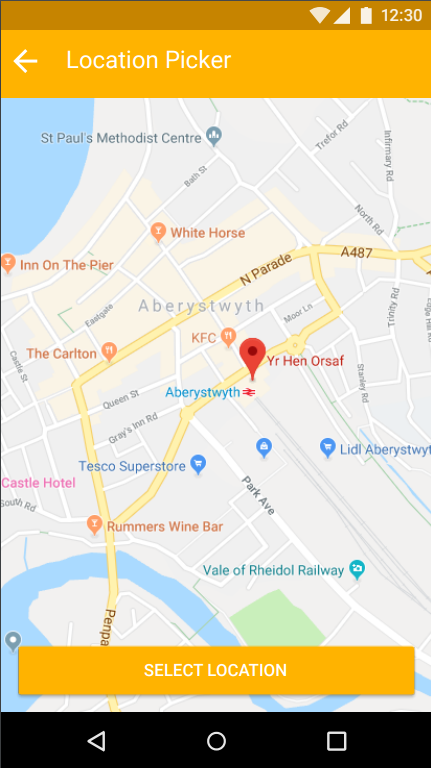
\includegraphics[width=0.5\linewidth]{Resources/img/location_picker_prototype.png}
	\caption{Prototype Screen for Picking Location via GPS}
	\label{fig:location_picker}
\end{figure}


\section{Conclusions}
This project was an invaluable learning experience. Both in terms of the technologies adopted and the project management aspects. The technologies and tools that were used worked together seamlessly. Given the modular nature of the platform, it is likely the case that any technology used for the API would integrate with the remainder of the platform with ease. The same is likely true for the choice of framework for the Web Application. However, having all the technologies be considered a common enough combination to have a designated acronym (MEAN stack) was certainly an encouraging sign.

The choice of Software Development Methodology was almost natural. The research into the correct way to implement an Extreme Programming approach paid off greatly. There was a bit of acclimatization required initially, and self-discipline to stick to the plan during each weekly cycle.